\documentclass[a4paper]{article}

\usepackage[english]{babel}
\usepackage[utf8]{inputenc}
\usepackage{amsmath}
\usepackage{graphicx}
\usepackage[colorinlistoftodos]{todonotes}

\title{Actividad 3}

\author{Jose Pablo Salazar Velazquez}

\date{febrero de 2016}

\begin{document}
\maketitle

\begin{abstract}
\end{abstract}

\section{Introduccion}
En el subcampo matemático del análisis numérico, se denomina interpolación a la obtención de nuevos puntos partiendo del conocimiento de un conjunto discreto de puntos.

En ingeniería y algunas ciencias es frecuente disponer de un cierto número de puntos obtenidos por muestreo o a partir de un experimento y pretender construir una función que los ajuste.

Otro problema estrechamente ligado con el de la interpolación es la aproximación de una función complicada por una más simple. Si tenemos una función cuyo cálculo resulta costoso, podemos partir de un cierto número de sus valores e interpolar dichos datos construyendo una función más simple. En general, por supuesto, no obtendremos los mismos valores evaluando la función obtenida que si evaluamos la función original, si bien dependiendo de las características del problema y del método de interpolación usado la ganancia en eficiencia puede compensar el error cometido.
En la Astronomía y navegación celeste, una efemérides proporciona las posiciones de los objetos astronómicos y satélites artificiales a un determinado tiempo. Históricamente, las posiciones se han proporcionado como tablas de valores, dados en intervalos regulares de fechas y tiempos. Las efemérides modernas se obtienen de modelos matemaáticos de los movimientos de los objetos astronómicos y la Tierra. 
 
 
Las efemérides han sido publicadas a lo largo de la historia de la humanidad, siendo las primeras efemérides en la cultura griega sobre el Cometa Halley alrededor de 466 AC, en  documentos de China y Babilonia. El cometa Halley se acerca al Sol cada 76-77 años. La última aparición fue en 1986 y la próxima oportunidad de observarlo será a mediados de 2061.
Para la creación  de los modelos matemáticos, es necesario encontrar una función que pase por todos los puntos observados. Eso se llama Interpolación.
 
En esta actividad aprenderemos un poco del proceso de encontrar una función que interpole todos los puntos, apoyados en la función scipy.interpolate de Python.

\section{Código}
\begin{verbatim}
import numpy as np
import matplotlib.pyplot as plt
from scipy.interpolate import interp1d

# Original "data set" --- 21 random numbers between 0 and 1.
x0 = np.linspace(-1,1,21)
y0 = np.random.random(21)

plt.plot(x0, y0, 'o', label='Data')

# Array with points in between those of the data set for interpolation.
x = np.linspace(-1,1,101)

# Available options for interp1d
options = ('linear', 'nearest', 'zero', 'slinear', 'quadratic', 'cubic', 10)

for o in options:
    f = interp1d(x0, y0, kind=o)    # interpolation function
    plt.plot(x, f(x), label=o)      # plot of interpolated data

plt.legend()
plt.show()
\end{verbatim}

\section{Resultados}
	\subsection{Dados 10 puntos aleatorios entre $x=0$ y $x=3$ para la función $f(x) = sin(2 x)$ .}
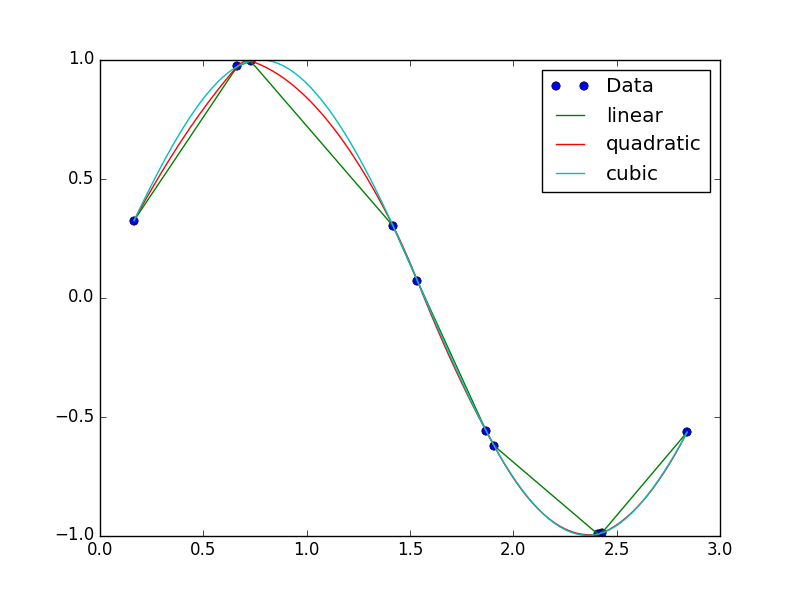
\includegraphics[width=11cm]{figure_1}
\\
\subsection{Dados 20 puntos aleatorios entre $x=-10$ y $x=10$ para la función $f(x) = sin(x)/x $}
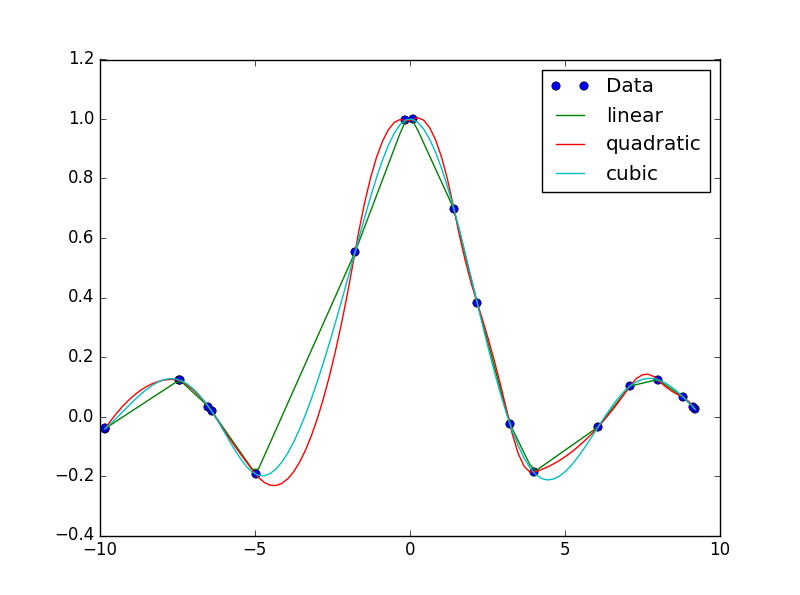
\includegraphics[width=11cm]{figure_2}
\\
\subsection{Dados 16 puntos aleatorios entre $x=-3$ y $x=3$ para la función $f(x) = x^2 sin(2 x)$}
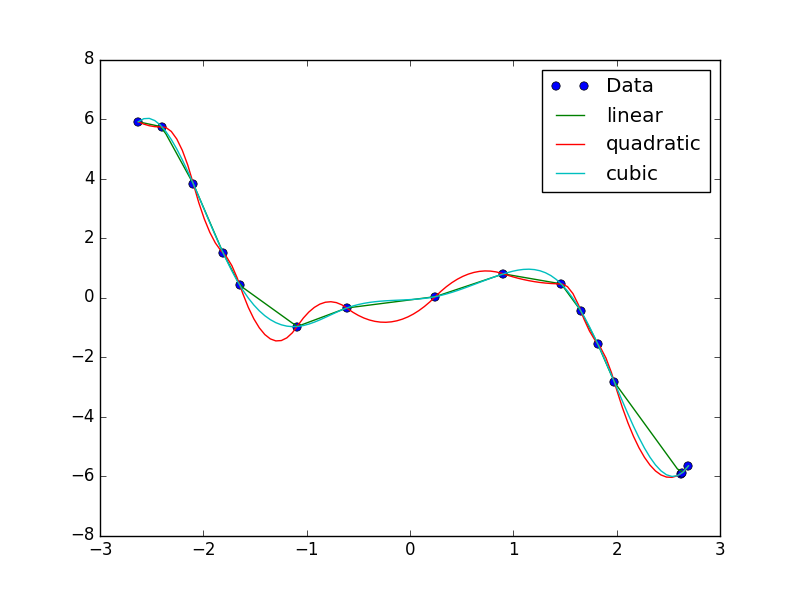
\includegraphics[width=11cm]{figure_3}
\\
\subsection{Dados 12 puntos aleatorios entre $x=-2$ y $x=2$ para la función $f(x) = x^3 sin(3 x)$}
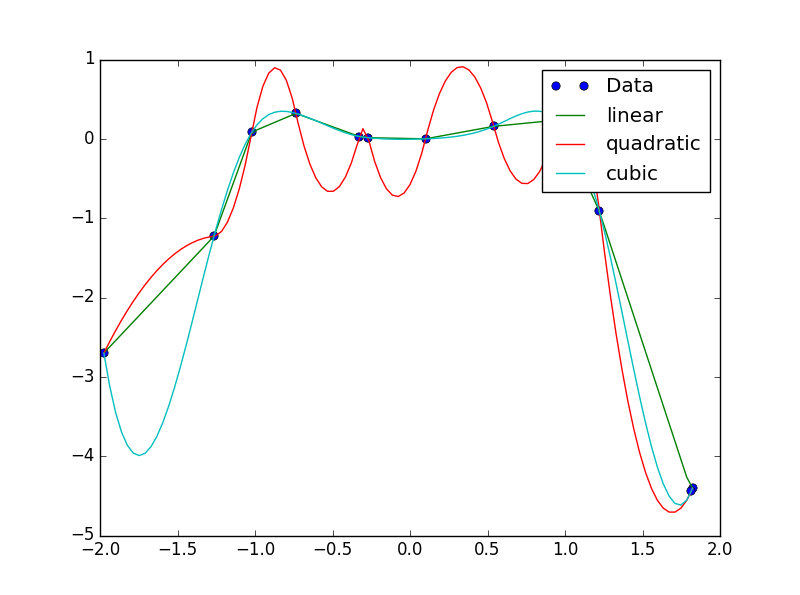
\includegraphics[width=11cm]{figure_4}
\end{document}